
%\subsection{Discussion}
%\label{sec:dsc}

%Let us look at both our techniques in the context of Zenger and Odersky 
%challenge to independently extensible solutions of extension problem discussed 
%in \textsection\ref{sec:exp}.

%\begin{itemize}
%\item Extensibility in both dimensions: \\
%      %It should be possible to add new data variants, while adapting the 
%      %existing operations accordingly. It should also be possible to introduce 
%      %new functions. 
%      Our techniques allow one to extend data with subclassing as well as 
%      introduce new functions through a match statement on corresponding 
%      encoding. The existing operations 
%\item Strong static type safety: \\
%      %It should be impossible to apply a function to a data variant, which it 
%      %cannot handle.
%\item No modification or duplication: \\
%      %Existing code should neither be modified nor duplicated.
%\item Separate compilation: \\
%      %Neither datatype extensions nor addition of new functions should require 
%      %re-typechecking the original datatype or existing functions. No safety 
%      %checks should be deferred until link or runtime.
%\item Independent extensibility: \\
%      %It should be possible to combine independently developed extensions so 
%      %that they can be used jointly.
%\end{itemize}
%
\section{Evaluation} %%%%%%%%%%%%%%%%%%%%%%%%%%%%%%%%%%%%%%%%%%%%%%%%%%%%%%%%%%%
\label{sec:eval}

We performed several independent studies of our approach to demonstrate its 
effectiveness. The first study compares our approach to the visitor design 
pattern and shows that the type switch is comparable or faster 
(\textsection\ref{sec:viscmp}). While we do not advocate for the closed solution 
of \textsection\ref{sec:cotc}, we included the comparison of type switching 
solutions made under open and closed world assumptions (\textsection\ref{sec:cmp}).
Our library supports both solutions with the same surface syntax, which is why 
we believe many users will try them both before settling on one.
The second study does a similar comparison with built-in facilities of Haskell 
and OCaml and shows that the open type switch for extensible and hierarchical 
data types can be almost as efficient as its equivalent for closed algebraic 
data types (\textsection\ref{sec:ocaml}). In the third study we looked at how 
well our caching mechanisms deal with some large real-world class hierarchies in 
order to demonstrate that our performance numbers were not established in overly 
idealistic conditions (\textsection\ref{sec:hierarchies}). In the last study we 
rewrote an existing visitor-based application using our approach in order to 
compare the ease of use, readability and maintainability of each approach, as 
well as to show the memory usage and the startup costs associated with our 
approach in a real application (\textsection\ref{sec:qualcmp}).

\subsection{Comparison with Visitor Design Pattern}
\label{sec:viscmp}

\begin{figure*}
\begin{tabular}{@{}c@{ }l||@{ }r@{}@{ }r@{}@{ }r@{}|@{ }r@{}@{ }r@{}@{ }r@{}||@{ }r@{}@{ }r@{}@{ }r@{}|@{ }r@{}@{ }r@{}@{ }r@{}||@{ }r@{}@{ }r@{}@{ }r@{}|@{ }r@{}@{ }r@{}@{ }r@{}}
\hline % -----------------------------------------------------------------------------------------------------------------------------------------
\hline % -----------------------------------------------------------------------------------------------------------------------------------------
 &            & \multicolumn{6}{c||}{G++/32 on Windows Laptop} & \multicolumn{6}{c||}{MS Visual C++/32}        & \multicolumn{6}{c}{MS Visual C++/64}           \\
\hline % -----------------------------------------------------------------------------------------------------------------------------------------
 & Syntax     & \multicolumn{3}{c|}{Unified} & \multicolumn{3}{c||}{Specialized} & \multicolumn{3}{c|}{Unified} & \multicolumn{3}{c||}{Specialized} & \multicolumn{3}{c|}{Unified} & \multicolumn{3}{c}{Specialized} \\
\hline % -----------------------------------------------------------------------------------------------------------------------------------------
 & Encoding   & \Opn  & \Cls  & \Unn  & \Opn  & \Cls  & \Unn  & \Opn  & \Cls  & \Unn  & \Opn  & \Cls  & \Unn  & \Opn  & \Cls  & \Unn  & \Opn  & \Cls  & \Unn   \\
\hline % -----------------------------------------------------------------------------------------------------------------------------------------
\hline % -----------------------------------------------------------------------------------------------------------------------------------------
 & Repetitive &\gwNGPp&\gwNGKp&\gwNGUp&\gwNSPp&\gwNSKp&\gwNSUp&\vwNGPp&\vwNGKp&\vwNGUp&\vwNSPp&\vwNSKp&\vwNSUp&\vxNGPp&\vxNGKp&\vxNGUp&\vxNSPp&\vxNSKp&\vxNSUp \\
 & Sequential &\gwNGPq&\gwNGKq&\gwNGUq&\gwNSPq&\gwNSKq&\gwNSUq&\vwNGPq&\vwNGKq&\vwNGUq&\vwNSPq&\vwNSKq&\vwNSUq&\vxNGPq&\vxNGKq&\vxNGUq&\vxNSPq&\vxNSKq&\vxNSUq \\
 & Random     &\gwNGPn&\gwNGKn&\gwNGUn&\gwNSPn&\gwNSKn&\gwNSUn&\vwNGPn&\vwNGKn&\vwNGUn&\vwNSPn&\vwNSKn&\vwNSUn&\vxNGPn&\vxNGKn&\vxNGUn&\vxNSPn&\vxNSKn&\vxNSUn \\
\hline % ------------------------------------------------------------------------------------------------------------------------------------------
\multirow{3}{*}{\begin{sideways}{\tiny Forward}\end{sideways}}
 & Repetitive &\gwYGPp&\gwYGKp&\gwYGUp&\gwYSPp&\gwYSKp&\gwYSUp&\vwYGPp&\vwYGKp&\vwYGUp&\vwYSPp&\vwYSKp&\vwYSUp&\vxYGPp&\vxYGKp&\vxYGUp&\vxYSPp&\vxYSKp&\vxYSUp \\
 & Sequential &\gwYGPq&\gwYGKq&\gwYGUq&\gwYSPq&\gwYSKq&\gwYSUq&\vwYGPq&\vwYGKq&\vwYGUq&\vwYSPq&\vwYSKq&\vwYSUq&\vxYGPq&\vxYGKq&\vxYGUq&\vxYSPq&\vxYSKq&\vxYSUq \\
 & Random     &\gwYGPn&\gwYGKn&\gwYGUn&\gwYSPn&\gwYSKn&\gwYSUn&\vwYGPn&\vwYGKn&\vwYGUn&\vwYSPn&\vwYSKn&\vwYSUn&\vxYGPn&\vxYGKn&\vxYGUn&\vxYSPn&\vxYSKn&\vxYSUn \\
\hline % -----------------------------------------------------------------------------------------------------------------------------------------
\hline % -----------------------------------------------------------------------------------------------------------------------------------------
 &            & \multicolumn{6}{c||}{G++/32 on Linux Desktop} & \multicolumn{6}{c||}{MS Visual C++/32 with PGO} & \multicolumn{6}{c}{MS Visual C++/64 with PGO} \\
\hline % -----------------------------------------------------------------------------------------------------------------------------------------
 & Syntax     & \multicolumn{3}{c|}{Unified} & \multicolumn{3}{c||}{Specialized} & \multicolumn{3}{c|}{Unified} & \multicolumn{3}{c||}{Specialized} & \multicolumn{3}{c|}{Unified} & \multicolumn{3}{c}{Specialized} \\
\hline % -----------------------------------------------------------------------------------------------------------------------------------------
 & Encoding   & \Opn  & \Cls  & \Unn  & \Opn  & \Cls  & \Unn  & \Opn  & \Cls  & \Unn  & \Opn  & \Cls  & \Unn  & \Opn  & \Cls  & \Unn  & \Opn  & \Cls  & \Unn   \\
\hline % -----------------------------------------------------------------------------------------------------------------------------------------
\hline % -----------------------------------------------------------------------------------------------------------------------------------------
 & Repetitive &\glNGPp&\glNGKp&\GwNGUp&\glNSPp&\glNSKp&\GwNSUp&\VwNGPp&\VwNGKp&\VwNGUp&\VwNSPp&\VwNSKp&\VwNSUp&\VxNGPp&\VxNGKp&\VxNGUp&\VxNSPp&\VxNSKp&\VxNSUp \\
 & Sequential &\glNGPq&\glNGKq&\GwNGUq&\glNSPq&\glNSKq&\GwNSUq&\VwNGPq&\VwNGKq&\VwNGUq&\VwNSPq&\VwNSKq&\VwNSUq&\VxNGPq&\VxNGKq&\VxNGUq&\VxNSPq&\VxNSKq&\VxNSUq \\
 & Random     &\glNGPn&\glNGKn&\GwNGUn&\glNSPn&\glNSKn&\GwNSUn&\VwNGPn&\VwNGKn&\VwNGUn&\VwNSPn&\VwNSKn&\VwNSUn&\VxNGPn&\VxNGKn&\VxNGUn&\VxNSPn&\VxNSKn&\VxNSUn \\
\hline % ------------------------------------------------------------------------------------------------------------------------------------------
\multirow{3}{*}{\begin{sideways}{\tiny Forward}\end{sideways}}
 & Repetitive &\glYGPp&\glYGKp&\GwYGUp&\glYSPp&\glYSKp&\GwYSUp&\VwYGPp&\VwYGKp&\VwYGUp&\VwYSPp&\VwYSKp&\VwYSUp&\VxYGPp&\VxYGKp&\VxYGUp&\VxYSPp&\VxYSKp&\VxYSUp \\
 & Sequential &\glYGPq&\glYGKq&\GwYGUq&\glYSPq&\glYSKq&\GwYSUq&\VwYGPq&\VwYGKq&\VwYGUq&\VwYSPq&\VwYSKq&\VwYSUq&\VxYGPq&\VxYGKq&\VxYGUq&\VxYSPq&\VxYSKq&\VxYSUq \\
 & Random     &\glYGPn&\glYGKn&\GwYGUn&\glYSPn&\glYSKn&\GwYSUn&\VwYGPn&\VwYGKn&\VwYGUn&\VwYSPn&\VwYSKn&\VwYSUn&\VxYGPn&\VxYGKn&\VxYGUn&\VxYSPn&\VxYSKn&\VxYSUn \\
\hline % -----------------------------------------------------------------------------------------------------------------------------------------
\hline % ----------------------------------------------------------------------------------------------------------------------------------
 &            & \multicolumn{6}{c||}{ } & \multicolumn{12}{c}{Windows Laptop}                                                      \\
\hline % ----------------------------------------------------------------------------------------------------------------------------------
\end{tabular}
\caption{Relative performance of type switching versus visitors. Numbers 
in regular font (e.g. \f{67}), indicate that our type switching is faster than 
visitors by corresponding percentage. Numbers in bold font (e.g. \s{14}), 
indicate that visitors are faster by corresponding percentage.}
\label{relperf}
\end{figure*}

Our comparison methodology involves several benchmarks representing various 
uses of objects inspected with either visitors or type switching.

The \emph{repetitive} benchmark (REP) performs calls on different objects of the 
same dynamic type. This scenario happens in object-oriented setting when a 
group of polymorphic objects is created and passed around (e.g. numerous 
particles of a given kind in a particle simulation system). We include it 
because double dispatch becomes twice faster (20 vs. 53 cycles) in this 
scenario compared to others due to hardware cache and call target prediction mechanisms. 

The \emph{sequential} benchmark (SEQ) effectively uses an object of each derived type only 
once and then moves on to an object of a different type. The cache is typically 
reused the least in this scenario, which is typical of lookup tables, where each 
entry is implemented with a different derived class.

The \emph{random} benchmark (RND) is the most representative as it randomly makes calls on 
different objects -- probably be the most common usage scenario in the real world.

Presence of \emph{forwarding} in any of these benchmarks refers to the 
common technique used by visitors where, for class hierarchies with multiple 
levels of inheritance, the \code{visit} method of a derived class will provide a 
default implementation of forwarding to its immediate base class, which, in turn, 
may forward it to its base class, etc. The use of forwarding in visitors is a 
way to achieve substitutability, which in type switch corresponds to the use 
of base classes in the case clauses.
This approach is used in Pivot, whose AST 
hierarchy consists of 154 node kinds, of which only 5 must be handled, while the 
rest will forward to them when visit for them was not overriden.

The class hierarchy for non-forwarding test was a flat hierarchy of 100 
derived classes, encoding an algebraic data type. The class hierarchy for 
forwarding tests had two levels of inheritance with 5 intermediate base classes 
and 95 derived ones. 

Each benchmark was tested with either \emph{unified} or \emph{specialized} 
syntax, each of which included tests on polymorphic (\emph{Open}) and tagged 
(\emph{Tag}) encodings. Specialized syntax avoids generating unnecessary 
syntactic structure used to unify syntax, and thus produces faster code. We 
include it in our results because a compiler implementation of type switching 
will only generate the best suitable code.

The benchmarks were executed in the following configurations referred to as 
\emph{Linux Desktop} and \emph{Windows Laptop} respectively:

\begin{itemize}
\setlength{\itemsep}{0pt}
\setlength{\parskip}{0pt}
\item \emph{Lnx}: Dell Dimension\textsuperscript{\textregistered} desktop with Intel\textsuperscript{\textregistered} Pentium\textsuperscript{\textregistered} 
      D (Dual Core) CPU at 2.80 GHz; 1GB of RAM; Fedora Core 13  
      \begin{itemize}
      \setlength{\itemsep}{0pt}
      \setlength{\parskip}{0pt}
      \item G++ 4.4.5 executed with -O2; x86 binaries
      \end{itemize}
\item \emph{Win}: Sony VAIO\textsuperscript{\textregistered} laptop with Intel\textsuperscript{\textregistered} Core\texttrademark i5 460M 
      CPU at 2.53 GHz; 6GB of RAM; Windows 7 Professional
      \begin{itemize}
      \setlength{\itemsep}{0pt}
      \setlength{\parskip}{0pt}
      \item G++ 4.6.1 / MinGW executed with -O2; x86 binaries
      \item MS Visual \Cpp{} 2010 Professional x86/x64 binaries with and without 
      Profile-Guided Optimizations
      \end{itemize}
\end{itemize}

\noindent
To improve accuracy, timing in all the configurations was performed with the 
help of \code{RDTSC} instruction available on x86 processors. For every number reported 
here we ran 101 experiments timing 1,000,000 dispatches each (all through either 
visitors or type switch). The first experiment was serving as a warm-up, during 
which the optimal caching parameters were inferred, and typically resulted in an 
outlier with the largest time. Averaged over 1,000,000 dispatches, the number of 
cycles per dispatch in each of the 101 experiments was sorted and the median was 
chosen. We preferred median to average to diminish the influence of other 
applications and OS interrupts as well as to improve reproducibility of timings 
between the runs of application. In particular, in the diagnostic boot of 
Windows, where the minimum of drivers and applications are loaded, we were 
getting the same number of cycles per iteration 70-80 out of 101 times. Timings 
in non-diagnostic boots had somewhat larger absolute values, however the 
relative performance of type switch against visitors remained unchanged and 
equally well reproducible.

\begin{figure}[htbp]
  \centering
    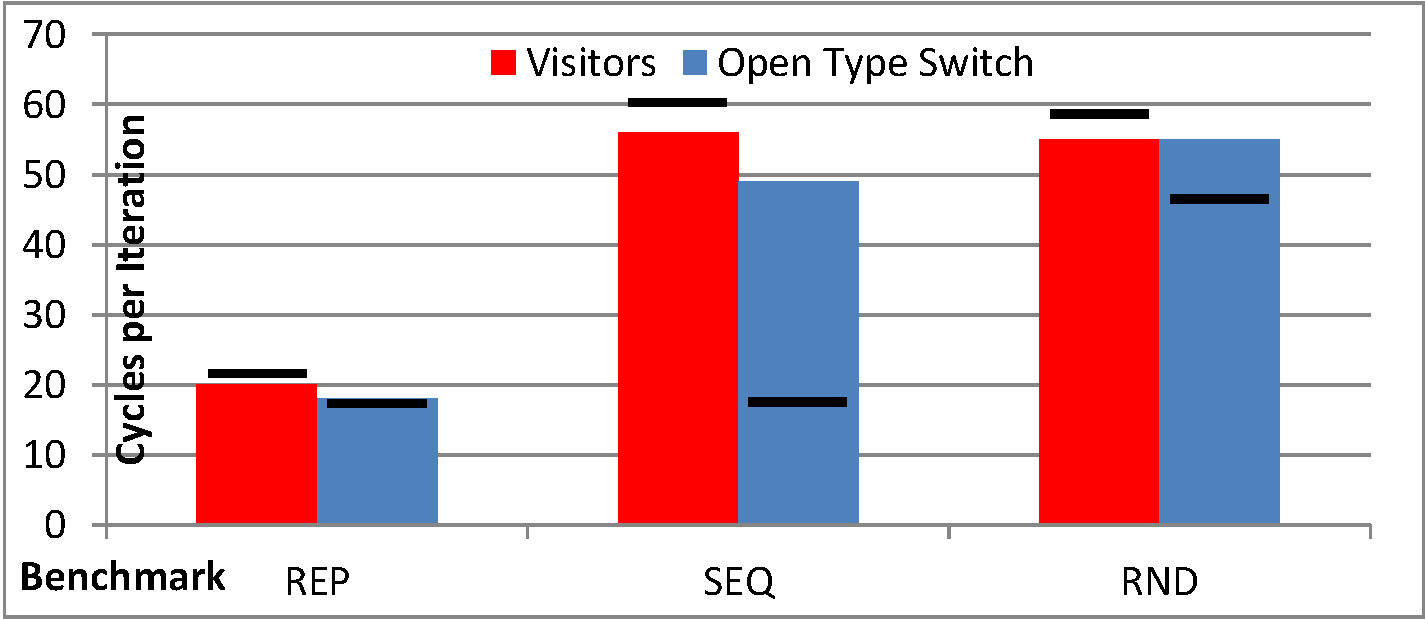
\includegraphics[width=0.47\textwidth]{VisitorsCompare.pdf}
  \caption{Absolute timings for different benchmarks}
  \label{fig:VisitorsComparison}
\end{figure}

To understand better the relative numbers of Figure~\ref{relperf}, we present 
in Figure~\ref{fig:VisitorsComparison} few absolute timings taken by visitors 
and open type switch to execute an iteration of a given benchmark. These absolute timings 
correspond to the relative numbers from column Open/G++/Win of Figure~\ref{relperf}.
The actual bars show the timings without forwarding, while the black lines 
indicate where the corresponding bar would be in the presence of forwarding. It 
is easy to see that visitors generally become slower in the presence of 
forwarding due to extra call, while type switch becomes faster due to smaller 
jump table. As discussed, both timings are much smaller for repetitive benchmark 
due to hardware cache.

Figure~\ref{relperf} provides a broader overview of how both techniques compare 
under different compiler/platform configurations. The values are given as 
percentages of performance increase against the slower technique. 
%Numbers in regular font represent cases where type switching was  
%faster, while underlined numbers in bold indicate cases where visitors were faster.

We can see that type switching wins by a good margin when implemented with tag switch (\textsection\ref{sec:cotc}) as  
well as in the presence of at least one level of forwarding. Note that the 
numbers are relative, and thus the ratio depends on both the performance of 
virtual function calls and the performance of switch statements. Visual \Cpp{} was 
generating faster virtual function calls, while GCC was generating faster switch 
statements, which is why their relative performance seem to be much more 
favorable for us in the case of GCC.
Similarly, the code for x86-64 is only slower relatively: the actual time spent for 
both visitors and type switching was smaller than that for x86-32, but it was much 
smaller for visitors than type switching, which resulted in worse relative 
performance.

The code on the critical path of our type switch implementation benefits 
significantly from branch hinting as some branches are much more likely than 
others. We use the branch hinting directives in GCC to guide the compiler, but, 
unfortunately, Visual \Cpp{} does not provide any similar facilities. Instead, 
Microsoft suggests using \emph{Profile-Guided Optimizations} (PGO) to achieve 
the same, which is why we list the results for Visual \Cpp{} both with and without 
profile-guided optimizations.
%The results without profile-guided optimizations can be 
%found in the accompanying technical report~\cite[\textsection 10]{TR}.
%The results of optimizing code created with Visual \Cpp{} by using profile 
%guided optimizations as currently Visual \Cpp{} does not have means for branch 
%hinting, which are supported by G++ and proven to be very effective in few 
%cruicial places. Profile guided optimization in Visual \Cpp{} lets compiler find 
%out experimentally what we would have otherwise hinted, even though this 
%includes other optimizations as well.

From the table it may seem that Visual C++ is generating not as good code as GCC 
does, but remember that these numbers are relative, and thus the ratio depends on  
both the performance of virtual calls and the performance of switch statements. Visual 
C++ was generating faster virtual function calls, while GCC was generating 
faster switch statements, which is why their relative performance seem to be much 
more favorable for us in the case of GCC.

Similarly the code for x64 is only slower relatively: the actual time spent for 
both visitors and type switching was smaller than that for x86, but it was much 
smaller for visitors than type switching, which resulted in worse relative 
performance.

\subsection{Open vs. Closed Type Switch}
\label{sec:cmp}

With only a few exceptions for x64, we saw in the Figure~\ref{relperf} that the 
performance of the closed tag switch (the Tag column) dominates the performance of the open type
swith (the Open column). We believe that the difference, often significant, is the price one pays 
for the true openness of the vtable pointer memoization solution.

As we mentioned in \textsection\ref{sec:cotc}, the use of tags, even when allocated 
by a compiler, may require integration efforts to ensure that different DLLs have 
not reused the same tags. Randomization of tags, similar to a proposal of 
Garrigue~\cite{garrigue-98}, will not eliminate the problem and will surely 
replace jump tables in switches with decision trees. This will likely 
significantly degrade the numbers for the part of Figure~\ref{relperf} 
representing closed tag switch, since the tags in our experiments were all 
sequential and small. 

The reliance of a tag switch on static cast, as described in \textsection\ref{sec:vtblmem}, this has severe limitations in the 
presence of multiple inheritance, and thus is not as versatile as open type 
switch. Overcoming this problem will either require the use of 
\code{dynamic_cast} or techniques similar to vtable pointer memoization, which 
will likely degrade tag switch's performance numbers even further.

Note also that the approach used to implement open type switch can be used to 
implement both first-fit and best-fit semantics, while the tag switch is only suitable 
for best-fit semantics. Their complexity guarantees also differ: open type 
switch is constant on average, but slow on the first call with given subobject. 
Tag switch is logarithmic in the size of the class hierarchy 
(assuming a balanced hierarchy), including the first call. This last point can 
very well be seen in Figure~\ref{relperf}, where the performance of a closed solution
degrades significantly in the presence of forwarding, while the performance of an
open solution improves.

\subsection{Comparison with OCaml and Haskell}
\label{sec:ocaml}

We now compare our solution to the built-in pattern-matching facility of 
OCaml~\cite{OPM01} and Haskell~\cite{Haskell98Book}.  
In this test, we timed small OCaml and Haskell applications performing our sequential 
benchmark on an algebraic data type of 100 variants. Corresponding \Cpp{} 
applications were working with a flat class hierarchy of 100 derived classes. 
The difference between the C++ applications lies in the encoding (Open/Tag/Kind) 
and the syntax (Unified/Special) used. Kind 
encoding is the same as Tag encoding, but it does not require substitutability, 
and thus can be implemented with a direct switch on tags without a ReMatch loop. 
It is only supported through specialized syntax in our library as it differs 
from the Tag encoding only semantically.

%The optimized OCaml compiler \texttt{ocamlopt.opt} that we used to compile the code 
%can be based on different toolsets on some platforms, e.g. Visual \Cpp{} or GCC 
%on Windows. To make the comparison fair we had to make sure that the 
%same toolset was used to compile the \Cpp{} code. We ran the tests 
%on both of the machines described above using the following configurations: 

%\begin{itemize}
%\setlength{\itemsep}{0pt}
%\setlength{\parskip}{0pt}
%\item The tests on a Windows 7 laptop were all based on the \emph{Visual \Cpp{} toolset} 
%      and used \texttt{ocamlopt.opt} version 3.11.0.
%\item The tests on a Linux desktop were all based on the \emph{GCC toolset} and used 
%      \texttt{ocamlopt.opt} version 3.11.2
%\end{itemize}

%\noindent
We used the optimizing OCaml compiler \texttt{ocamlopt.opt} version 3.11.0 working 
under the Visual \Cpp{} toolset as well as the Glasgow Haskell Compiler version 
7.0.3 (with -O switch) working under the MinGW toolset. The \Cpp{} applications 
were compiled with Visual \Cpp{} as well and all the tests were  
performed on the Windows 7 laptop. Similar to comparison with visitors,
the timing results presented in Figure~\ref{fig:OCamlComparison} are averaged 
over 101 measurements and show the number of seconds it took to perform a 
1,000,000 decompositions within our sequential benchmark. We compare here time 
and not cycles, as that was the only common measurement in all three 
environments.

\begin{figure}[htbp]
  \centering
    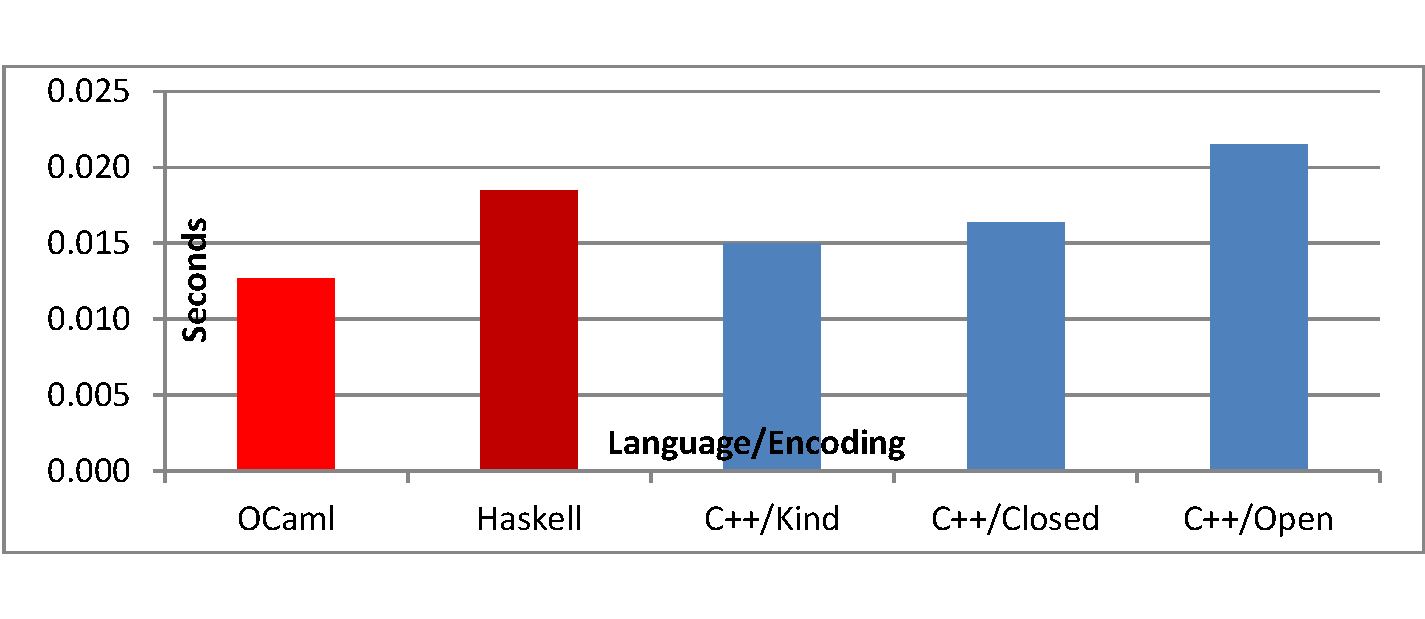
\includegraphics[width=0.47\textwidth]{OCamlComparison.pdf}
  \caption{Performance comparison with OCaml \& Haskell}
  \label{fig:OCamlComparison}
\end{figure}

We can see that the use of specialized syntax on a closed/sealed hierarchy can 
match the speed of, and even be four times faster than, the code generated by 
the native OCaml compiler. Once we go for an open solution, we become about 
30-50\% slower. 

\subsection{Dealing with real-world class hierarchies}
\label{sec:hierarchies}

For this experiment, we used a class hierarchy benchmark previously used in the 
literature to study efficiency of type inclusion testing and dispatching 
techniques~\cite{Vitek97,Krall97nearoptimal,PQEncoding,Ducournau08}.
We use the names of each benchmark from Vitek et al~\cite[Table 2]{Vitek97}, 
since the set of benchmarks we were working with was closest (though not exact) 
to that work.

While not all class hierarchies originated from \Cpp{}, for this experiment it 
was more important for us that the hierarchies were man-made. While converting 
the hierarchies into \Cpp{}, we had to prune inaccessible base classes (direct base  
class that is already an indirect base class) when used with repeated 
inheritance in order to satisfy semantic requirements of \Cpp{}. We maintained 
the same number of virtual functions present in each class as well as the number 
of data members; the benchmarks, however, did not preserve the exact types of those.
The data in Figure~\ref{fig:benchmarks} shows various parameters of the class 
hierarchies in each benchmark, after their adoption to \Cpp{}. 

\begin{figure}[htbp]
\footnotesize
\begin{tabular}{@{ }l@{ }||@{ }l@{ }|@{ }r@{ }|@{ }r@{ }|@{ }r@{ }|@{ }r@{ }|@{ }r@{ }|@{ }r@{ }|@{ }l@{ }|@{ }r@{ }|@{ }r@{ }|@{ }r@{ }}
\hline % --------------------------------------------------------------------------------------------------
\multicolumn{1}{@{}c@{}||}{\multirow{2}{*}{\tiny{\textsc{Library}}}} & 
\multicolumn{1}{@{ }c@{ }|}{\multirow{2}{*}{\tiny{\textsc{Language}}}} & 
\multicolumn{1}{@{ }c@{ }|}{\multirow{2}{*}{\tiny{\textsc{Classes}}}} &
\multicolumn{1}{@{ }c@{ }|}{\multirow{2}{*}{\tiny{\textsc{Paths}}}} & 
\multicolumn{1}{@{ }c@{ }|}{\multirow{2}{*}{\tiny{\textsc{Height}}}} & 
\multicolumn{1}{@{ }c@{ }|}{\multirow{2}{*}{\tiny{\textsc{Roots}}}} & 
\multicolumn{1}{@{ }c@{ }|}{\multirow{2}{*}{\tiny{\textsc{Leafs}}}} & 
\multicolumn{1}{@{ }c@{ }|}{\multirow{2}{*}{\tiny{\textsc{Both}}}} & 
\multicolumn{2}{@{}c@{}|}{\tiny{\textsc{Parents}}} & 
\multicolumn{2}{@{}c@{}}{\tiny{\textsc{Children}}} \\ \cline{9-12}
     &                             &      &       &    &     &      &     & \multicolumn{1}{@{}c@{}|}{\tiny{\textsc{avg}}} & \multicolumn{1}{@{}c@{}|}{\tiny{\textsc{max}}} & \multicolumn{1}{@{}c@{}|}{\tiny{\textsc{avg}}} & \multicolumn{1}{@{}c@{}}{\tiny{\textsc{max}}} \\
\hline % --------------------------------------------------------------------------------------------------
 DG2 & \tiny{\textsc{Smalltalk}}   &  534 &   534 & 11 &   2 &  381 &   1 & 1    &  1 & 3.48 &  59 \\ % digitalk2         
 DG3 & \tiny{\textsc{Smalltalk}}   & 1356 &  1356 & 13 &   2 &  923 &   1 & 1    &  1 & 3.13 & 142 \\ % digitalk3         
 ET+ & \tiny{\textsc{\Cpp{}}}      &  370 &   370 &  8 &  87 &  289 &  79 & 1    &  1 & 3.49 &  51 \\ % et++              
 GEO & \tiny{\textsc{Eiffel}}      & 1318 & 13798 & 14 &   1 &  732 &   0 & 1.89 & 16 & 4.75 & 323 \\ % geode             
 JAV & \tiny{\textsc{Java}}        &  604 &   792 & 10 &   1 &  445 &   0 & 1.08 &  3 & 4.64 & 210 \\ % java              
 LOV & \tiny{\textsc{Eiffel}}      &  436 &  1846 & 10 &   1 &  218 &   0 & 1.72 & 10 & 3.55 &  78 \\ % lov-object-editor 
 NXT & \tiny{\textsc{Objective-C}} &  310 &   310 &  7 &   2 &  246 &   1 & 1    &  1 & 4.81 & 142 \\ % nextstep          
 SLF & \tiny{\textsc{Self}}        & 1801 & 36420 & 17 &  51 & 1134 &   0 & 1.05 &  9 & 2.76 & 232 \\ % self              
 UNI & \tiny{\textsc{\Cpp{}}}      &  613 &   633 &  9 & 147 &  481 & 117 & 1.02 &  2 & 3.61 &  39 \\ % unidraw           
%    &                             &   51 &    51 &  7 &   1 &   29 &   0 & 1.00 &  1 & 2.27 &   5 \\ % v1-collection     
%    &                             &   18 &    18 &  5 &   1 &   11 &   0 & 1.00 &  1 & 2.43 &   5 \\ % v1-magnitude      
%    &                             &  383 &   383 &  9 &   1 &  244 &   0 & 1.00 &  1 & 2.75 &  86 \\ % v1-object-nometa  
%    &                             &    9 &     9 &  5 &   1 &    4 &   0 & 1.00 &  1 & 1.60 &   2 \\ % v1-set            
%    &                             &   16 &    16 &  7 &   1 &    7 &   0 & 1.00 &  1 & 1.67 &   2 \\ % v1-stream         
%    &                             &   53 &    53 &  8 &   1 &   31 &   0 & 1.00 &  1 & 2.36 &   7 \\ % v1-visualcomponent
 VA2$_a$& \tiny{\textsc{Smalltalk}}& 3241 &  3241 & 14 &   1 & 2582 &   0 & 1    &  1 & 4.92 & 249 \\ % visualage2.all    
 VA2$_k$& \tiny{\textsc{Smalltalk}}& 2320 &  2320 & 13 &   1 & 1868 &   0 & 1    &  1 & 5.13 & 240 \\ % visualage2.kern   
 VW1 & \tiny{\textsc{Smalltalk}}   &  387 &   387 &  9 &   1 &  246 &   0 & 1    &  1 & 2.74 &  87 \\ % visualworks1      
 VW2 & \tiny{\textsc{Smalltalk}}   & 1956 &  1956 & 15 &   1 & 1332 &   0 & 1    &  1 & 3.13 & 181 \\ % visualworks2      
%    &                             &    6 &     9 &  4 &   2 &    1 &   0 & 1.50 &  2 & 1.20 &   2 \\ % vtbl              
\hline % --------------------------------------------------------------------------------------------------
\multicolumn{2}{r|}{\tiny{\textsc{Overalls}}} &15246 & 63963 & 17 & 298 &10877 & 199 & 1.11 & 16 & 3.89 & 323 \\ % Overalls
\hline % --------------------------------------------------------------------------------------------------
\end{tabular}
\caption{Benchmark class hierarchies}
\label{fig:benchmarks}
\end{figure}

The number of paths represents the number of distinct inheritance paths from the 
classes in the hierarchy to the roots of the hierarchy. This number reflects the number of possible subobjects in the 
hierarchy. The roots listed in the table are classes with no base classes. We 
will subsequently use the term \emph{non-leaf} to refer to the possible root of 
a subhierarchy. Leafs are classes with no children, while \emph{both} refers to 
utility classes that are both roots and leafs and thus neither have base nor 
derived classes. The average for the number of parents and the number of 
children were computed only among the classes having at least one parent or at 
least one child correspondingly.

With few useful exceptions, it generally makes sense to apply type switch only 
to non-leaf nodes of the class hierarchy. 71\% of the classes in the entire 
benchmarks suite were leaf classes. Out of the 4369 non-leaf classes, 36\% were 
spawning a subhierarchy of only 2 classes (including the root), 15\% -- a 
subhierarchy of 3 classes, 10\% of 4, 7\% of 5 and so forth. 
Turning this into a cumulative distribution, $a\%$ of subhierarchies had more 
than $b$ classes in them:

%\noindent
\begin{tabular}
{l||@{ }c@{ }|@{ }c@{ }|@{ }c@{ }|@{ }c@{ }|@{ }c@{ }|@{ }c@{ }|@{ }c@{ }|@{ }c@{ }|@{ }c@{ }}
%{l||c|c|c|c|c|c|c|c|c}
$a$ & 1\% & 3\% & 5\% & 10\% & 20\% & 25\% & 50\% & 64\% & 100\% \\
\hline % --------------------------------------------------------------------------------------------------
$b$ & 700 & 110 & 50  & 20   & 10   & 7    & 3    & 2    & 1
\end{tabular}

%1\% of subhierarchies had more than 700 classes in them, 3\% of subhierarchies 
%had more than 110 classes, 5\% of subhierarchies had more than 50 classes, 10\% 
%of subhierarchies had more than 20 classes, 20\% of subhierarchies had more than 
%10 classes, 25\% of hierarchies had more than 7 classes, only 50\% of 
%hierarchies had more than 3 classes and 64\% -- more than 2.

\noindent
These numbers reflect the percentage of use cases one may expect in the real 
word that have a given number of case clauses in them.

For each non-leaf class $A$ we created a function performing a type switch on 
every possible derived class $D_i$ of it as well as itself. The function was 
then executed with every possible subobject $D_i\leftY\sigma_j\rightY A$ it can  
possibly be applied to, given the static type $A$ of the subject. It was 
executed multiple but the same number of times on each subobject to ensure 
uniformity on one side (since we do not have the data about the actual 
probabilities of each subobject in the benchmark hierarchies) as well as let the 
type switch infer the optimal parameters $k$ and $l$ of its cache indexing 
function $H_{kl}^V$. We then plotted a point in chart of Figure~\ref{fig:prob} 
relating 2 characteristics of each of the 4396 type switches tested: the optimal 
computed probability of conflict $p$ achieved by the type switch and the number 
of subobjects $n$ that came through that type switch. The actual frequencies of 
collisions were within one tenth of a percentage point of the computed 
probabilities, which is why we did not use them in the chart. To account for the 
fact that multiple experiments could have resulted in the same pair $(n,p)$, we 
use a shadow of each point to reflect somewhat the number of experiments 
yielding it.

\begin{figure}[htbp]
  \centering
    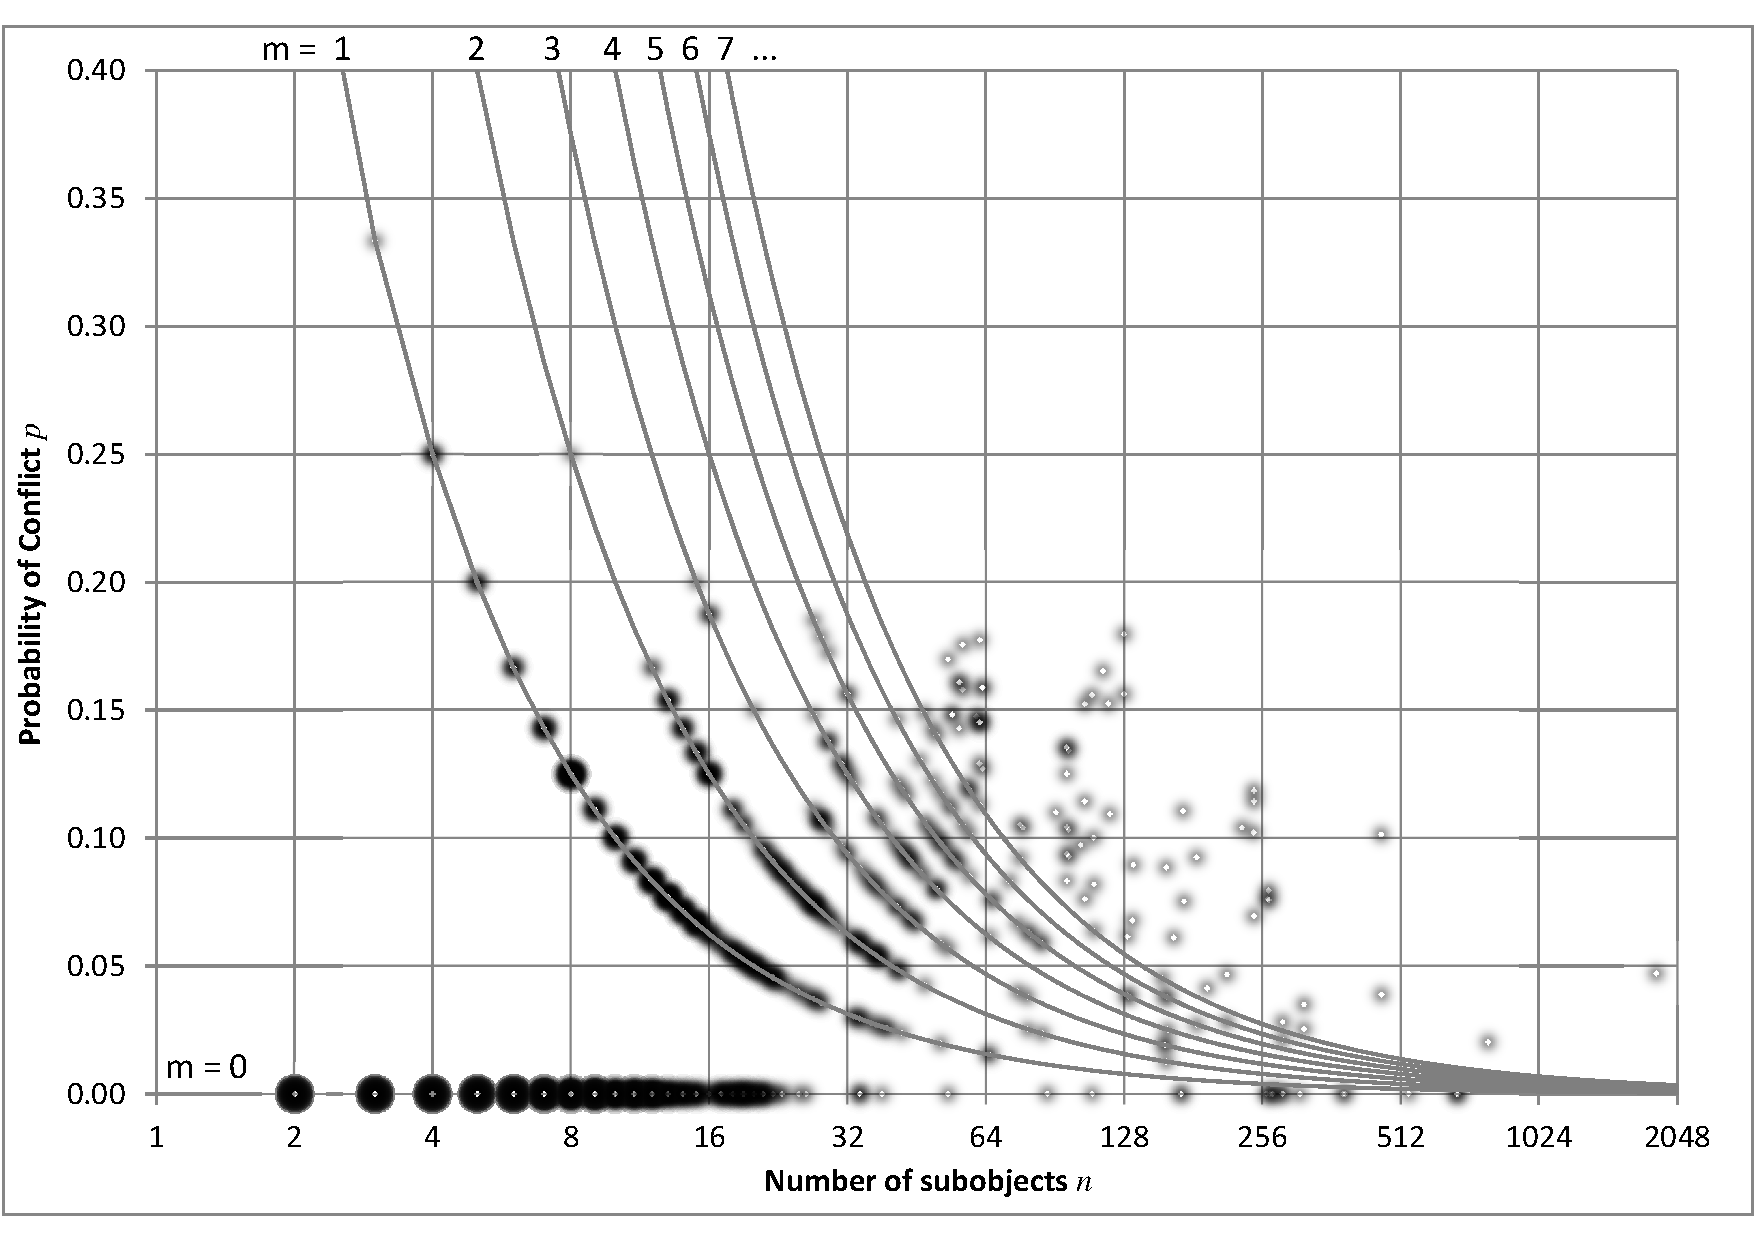
\includegraphics[width=0.49\textwidth]{ClassHierarchies.pdf}
  \caption{Probability of conflict in real hierarchies}
  \label{fig:prob}
\end{figure}

The curves on which the results of experiments line up correspond to the fact 
that under uniform distribution of $n$ subobjects, only a finite number of 
different values representing the probability of conflict $p$ is possible. In 
particular, all such values $p=\frac{m}{n}$, where $0 \le m < n$. The number $m$ 
reflects the number of subobjects an optimal cache indexing function $H_{kl}^V$ 
could not allocate their own entry for and we showed in \textsection\ref{sec:moc} 
that the probability of conflict under uniform distribution of $n$ subobjects 
depends only on $m$. The curves thus correspond to graphs of functions 
$y=\frac{m}{x}$ for different values of $m$. The points on the same curve (which 
becomes a line on a log-log plot) all share the same number $m$ of ``extra'' 
vtbl-pointers that optimal cache indexing function could not allocate individual 
entries for.

While it is hard to see from the chart, 87.5\% of all the points on the chart 
lay on the X-axis, which means that the optimal hash function for the 
corresponding type switches had no conflicts at all ($m=0$). In other words, only in 12.5\% 
of cases the optimal $H_{kl}^V$ for the set of vtbl-pointers $V$ coming through 
a given type switch had non-zero probability of conflict. Experiments laying on 
the first curve amount to 5.58\% of subhierarchies and represent the cases in 
which optimal $H_{kl}^V$ had only one ``extra'' vtbl-pointer ($m=1$). 2.63\% of 
experiments had $H_{kl}^V$ with 2 conflicts, 0.87\% with 3 and so forth as shown 
in Figure~\ref{fig:size}($K+1$).

\begin{figure}[htbp]
\small
\begin{tabular}
{@{}c@{}||@{}c@{ }|@{}c@{ }|@{}c@{ }|@{}c@{ }|@{}c@{ }|@{}c@{ }|@{}c@{ }|@{}c@{ }}
\hline % -------------------------------------------------------------------------
  $m$ &       0 &       1 &      2 &      3 &      4 &        5 &      6 & \textgreater 6 \\
\hline % -------------------------------------------------------------------------
$K+1$ & 87.50\% &  5.58\% & 2.63\% & 0.87\% & 0.69\% & 0.69\% & 0.30\% & 1.76\% \\
\hline % -------------------------------------------------------------------------
  $K$ & 72.55\% & 12.27\% & 4.87\% & 2.61\% & 1.42\% & 0.94\% & 0.80\% & 4.55\% 
\end{tabular}
\caption{Percentage of type switches with given number of conflicts ($m$) under different size constraints}
\label{fig:size}
\end{figure}

In cases when the user is willing to trade performance for better space 
efficiency she may restrict $k$ to $[K,K]$ instead of $[K,K+1]$ as discussed in 
\textsection\ref{sec:moc}. We redid all the 4396 experiments under this 
restriction and obtained a similar histogram shown in Figure~\ref{fig:size}($K$).
The average probability of conflict over the entire set increased from 0.011 to 
0.049, while the maximum probability of conflict increased from 0.333 to 0.375. 
The average load factor of the cache expectedly increased from 75.45\% to 82.47\%. 

It is important to understand that the high ratio of cases in which the hash 
function could deliver perfect indexing does not indicate that the hash function 
we used is better than other hash functions. It does indicate instead that the 
values representing vtbl-pointers in a given application are not random at all and 
are particularly suitable for such a hash function.

\subsection{Refactoring an existing visitors based application}
\label{sec:qualcmp}

For this experiment, we reimplemented a visitor based \Cpp{} pretty printer for 
Pivot\cite{Pivot09} using \emph{Mach7}. The Pivot's class hierarchy 
consists of 154 node kinds representing various entities in the \Cpp{} program. The 
original code had 8 visitor classes each handling 5, 7, 8, 10, 15, 17, 30 and 63 
cases, which we turned into 8 match statements with corresponding numbers of 
case clauses. Most of the rewrite was performed by sed-like replaces that 
converted visit methods into respective case-clauses. In several cases we had to 
manually reorder case-clauses to avoid redundancy as visit-methods for base classes 
were typically coming before the same for derived, while for type switching we 
needed them to come after due to first-fit semantics. Redundancy checking 
support provided by \emph{Mach7} and discussed in \textsection\ref{sec:redun} was invaluable in finding all such cases.

During this refactoring we have made several simplifications that became obvious 
in pattern-matching code, but were not in visitors code because of control 
inversion. Simplifications that were applicable to visitors code were eventually 
integrated into visitors code as well to make sure we do not compare 
algorithmically different code. In any case we were making sure that both 
approaches regardless of simplifications were producing byte-to-byte the same 
output as the original pretty printer we started from.

The size of executable for pattern-matching approach was smaller than that for 
visitors. So was also the source code. We extracted from both sources the 
functionality that was common to them and placed it in a separate translation 
unit to make sure it does not participate in the comparison. We kept all the 
comments however that were eqaully applicable to code in either approach.

Both pretty printers were executed on a set of header files from the \Cpp{} 
standard library and the produced output of both program was byte-to-byte the same. 
We timed execution of the pretty printing phase (not including loading and termination 
of the application or parsing of the source file) and observed that on small 
files (e.g. those from C run-time library and few small \Cpp{} files) 
visitors-based implementation was faster because the total number of nodes in 
AST and thus calls did not justify our set-up calls. In particular, 
visitor-based implementation of the pretty printer was faster on files of 44--588  
lines of code, with average 136 lines per those inputs, where visitors win. On 
these input files, visitors are faster by 1.17\%--21.42\% with an average speed-up of 
8.75\%. Open type switch based implementation of the pretty printer was faster on 
files of 144--9851 lines of code, with average 3497 lines per those input files, 
where open type switch wins. On these inputs, open type switch is faster by 0.18\% -- 32.99\% 
with an average speed-up of 5.53\%.

Figure~\ref{fig:mem} shows memory usage as well as cache hits and misses for 
the run of our pretty printer on \code{<queue>} standard library 
header, which had the largest LOC count after preprocessing in our test set.

\begin{figure}[htbp]
  \centering
    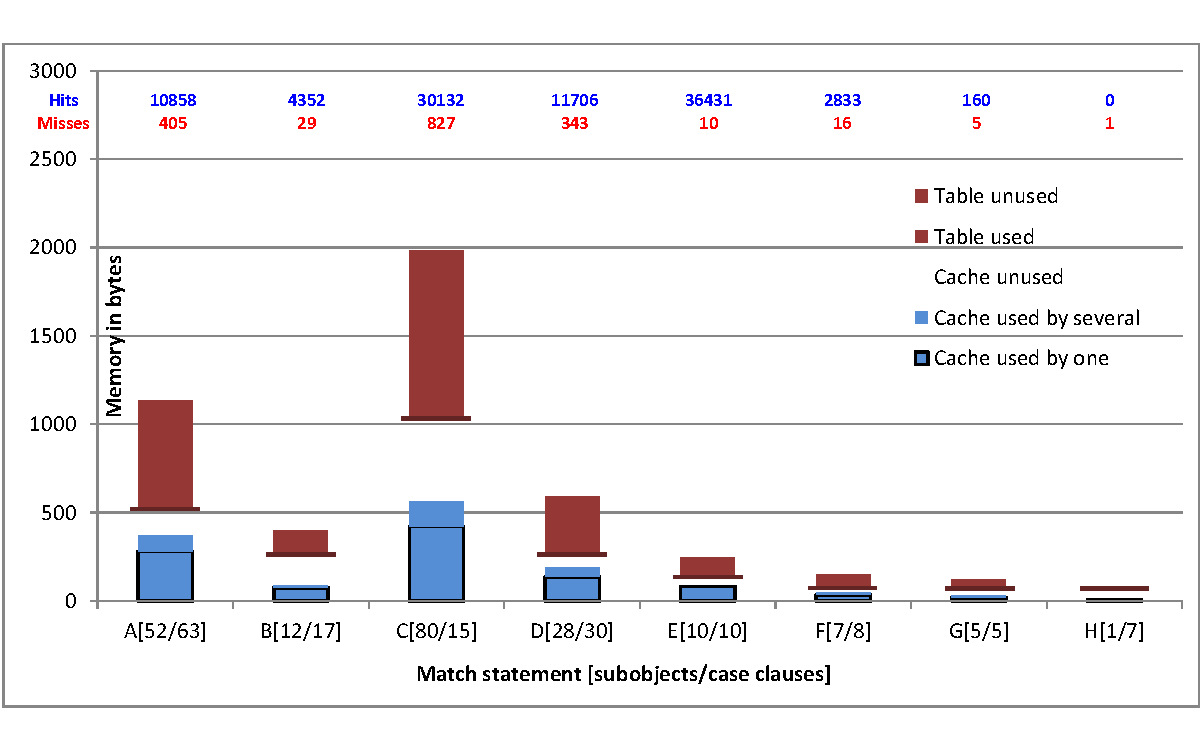
\includegraphics[width=0.49\textwidth]{Memory.pdf}
  \caption{Memory usage in real application}
  \label{fig:mem}
\end{figure}

The bars represent the total size of memory in bytes each of the 8 match 
statements (marked A-H) used. Information $[n/c]$ next to the letter indicates the 
actual number of different subobjects (i.e. vtbl-pointers) $n$ that came through 
that match statement, and the number of case clauses $c$ the match statement had 
(the library uses $c$ as an estimate of $n$). $n$ is also the number of cases the 
corresponding match statement had to be executed sequentially (instead of a 
direct jump).

The lower part of each bar (with respect to dividing line) corresponds to the memory used by cache, while the 
upper part -- to the memory used by the hash table. The ratio of the darker
section of each part to the entire part indicates the load factors 
of cache and hash-table respectively. The black box additionally indicates the 
proportion of cache entries that are allocated for only one vtbl-pointer and 
thus never result in a cache miss. %The non-transparent part without black box 
%represents the percentage of vtbl-pointers that have to share their cache entry 
%with at least one other vtbl-pointer and thus may result in collisions during 
%access.

The actual number of hits and misses for each of the match statements is 
indicated on top of the corresponding column. The sum of them is the total 
number of calls made. %Hits indicate situation when we found entry in cache and 
%didn't have to make roundtrip to the hash-table to get it. Misses indicate the 
%number of cases during actual run we had to pick the entry from the hash table 
%and update the cache with it. 
The number of misses is always larger than or equal to $n$ since we need to 
execute the switch sequentially on each of them once in order to memoize the 
outcome.

The library always preallocates memory for at least 8 subobjects to avoid 
unnecessary recomputations of optimal parameters $k$ and $l$ -- this is the case 
with the last 3 match statements. In all other cases it allocates the 
memory proportional to $2^{K+1}$ where $2^{K-1} < \max(n,c) \le 2^{K}$. We make 
$c$ a parameter, because in a library setting $n$ is not known up front and 
estimating it with $c$ allows us to avoid unnecessary recomputations of $l$ and 
$k$ even further. 

The table does not have to be hash table and can be implemented with 
any other container i.e. sorted vector, map etc. that let us find quickly by a given 
vtbl-pointer the data associated with it. In fact we provide a slightly less 
efficient caching container that avoids the table altogether, thus significantly 
reducing the memory requirements instead.

%During this refactoring we have made several simplifications that became obvious 
%in pattern-matching code, but were not in visitors code because of control 
%inversion. Simplifications that were applicable to visitors code were eventually 
%integrated into visitors code as well to make sure we do not compare 
%algorithmically different code. In any case we were making sure that both 
%approaches regardless of simplifications were producing byte-to-byte the same 
%output as the original pretty printer we started from.

%The size of executable for pattern-matching approach was smaller than that for 
%visitors. So was also the source code. We extracted from both sources the 
%functionality that was common to them and placed it in a separate translation 
%unit to make sure it does not participate in the comparison. We kept all the 
%comments however that were eqaully applicable to code in either approach.
%
Note that the visitors involved in the pretty printer above did not use 
forwarding: since all the \Cpp{} constructs were handled by the printer, every 
visit-method was overriden from those statically possible based on the static 
type of the argument.

Listing parameter for a case clause always causes access to member. Best hope is 
that compiler will eliminate it if it is not needed. At the moment we do not 
have means to detect empty macro arguments or \_.

In general from our rewriting experience we will not recommend rewriting 
existing visitor code with pattern matching for the simple reason that pattern 
matching code will likely follow the structure already set by the visitors. 
Pattern matching was most effective when writing new code, where we could design 
the structure of the code having the pattern-matching facility in our toolbox.

\subsection{Limitations}
\label{sec:lim}

Currently the definition of each class used in a case clause must be visible to 
the compiler because \code{dynamic_cast} operator used in the type switch does 
not allow incomplete types as a target type. For particularly large type 
switches (e.g. \textgreater 1000 case clauses) this may easily reach some 
compiler limitations. Both GCC and Visual \Cpp{}, for example, could not generate 
object files for such translation units simply because the sheer size of v-tables 
and other compiler data in it were exceeding the limits. The problem is not 
specific to our technique though and allowing \code{dynamic_cast} on classes 
that were declared but not defined yet would solve the problem.

While it might be reasonable to expect from linkers to layout v-tables close 
to each other -- the property that makes our hashing function efficient -- they 
are not required to do so. We believe, nevertheless, that should our approach 
become popular through the library implementation, its compiler implementation 
will encourage compiler vendors to enforce the property in order to keep the 
type switching fast.
